\section{State-Of-The-Art by Example: The API and Structure of LMFDB}\label{sec:sota}

L-functions and Modular Forms Database \cite{lmfdb}, or \lmfdb\ for short, is a project is a mathematical database. 
It is implemented in Python with a MongoDB backend. 
The project contains several thousand L-Functions and curves along with their properties. 

We use this as an example of a Virtual Theory. 
Before we go into this in more detail, we first have a closer look at the structure and existing APIs to communicate with it. 

\subsection{The Structure of LMFDB}\label{sec:sota:struct}

\lmfdb\ has several sub-databases - each of which contains different kinds of objects. 
These databases include e.g. a database of elliptic curves or a database of transitive groups. 

\begin{figure}[h]
  \begin{center}
      \begin{lstlisting}[language=json]
{
    "degree": 1,
    "non-maximal_primes": [5],
    "torsion_structure": ["5"],
    "ainvs": ["0","-1","1","-10","-20"],
    "x-coordinates_of_integral_points": "[5,16]",
    "real_period": 1.26920930427955,
    "min_quad_twist": {"disc": 1,"label": "11a1"},
    "sha_an": 1.0,
    "conductor": 11,
    "iwp0": 7,
    "2adic_gens": [],
    "torsion_primes": [5],
    "signD": -1,
    "tamagawa_product": 5,
    "isogeny_matrix": [[1,5,25],[5,1,5],[25,5,1]],
    "non-surjective_primes": [5],
    "lmfdb_label": "11.a2",
    "2adic_index": 1,
    "equation": "\\( y^2 + y = x^{3} -  x^{2} - 10 x - 20  \\)",
    "label": "11a1",
    "regulator": 1.0,
    "anlist": [0,1,-2,-1,2,1,2,-2,0,-2,-2,1,-2,4,4,-1,-4,-2,4,0,2],
    "iso": "11a",
    "_id": "ObjectId('4f71d4304d47869291435e6e')"
}
      \end{lstlisting}
  \end{center}
  
  \vspace*{-1.5em}
  

  \caption[An elliptic curve within lmfdb]{
    An elliptic curve, as found within \lmfdb. 
    Some key-value pairs are omitted for readability. 
  }
  \label{fig:lmfdbexample}
\end{figure}

Within each database, each curve is stored as a single JSON object with common keys. 
An example of a single entry in the elliptic curve can be seen in Figure~\ref{fig:lmfdbexample}.

When a mathematician looks at this representation of a curve, they can be easily confused; it is not immediately obvious which mathematical object is depicted here. 
After a closer look, it becomes clear that this curve is shown as a record, i.e. a mapping from keys (in this case strings) to values (any kind of JSON values). 

This leads to the conclusion that each property of this JSON object has to correspond to a single property of the underlying mathematical object. 
For example, the \identifier{degree} property -- here $1$ -- of the JSON objects corresponds to the degree of the underlying elliptic curve. 

Other properties are more complicated. 
Whereas the value of the \identifier{degree} property is a simple integer, the value of the \identifier{isogeny\_matrix} property is a list of lists. 
Obviously, as a mathematician this is to be interpreted as a matrix. 
This can become even more technical. 
For example the \identifier{x-coordinates\_of\_integral\_points} field, \lmfdb\ represents a list of integers as a list of strings.

\subsection{An API for LMFDB Objects}\label{sec:sota:api}

This already shows that it is non-trivial to get from a representation of elliptic curve inside of \lmfdb\ to a mathematical object. 
However, being a mathematical knowledge base, one use case of \lmfdb\ is to find elliptic curves subject to specific criteria. 
As a very simple example, suppose a mathematician wants to find all abelian elliptic curves. 
How can this be achieved using the \lmfdb\ API?

\begin{figure}[h]
  \begin{center}
    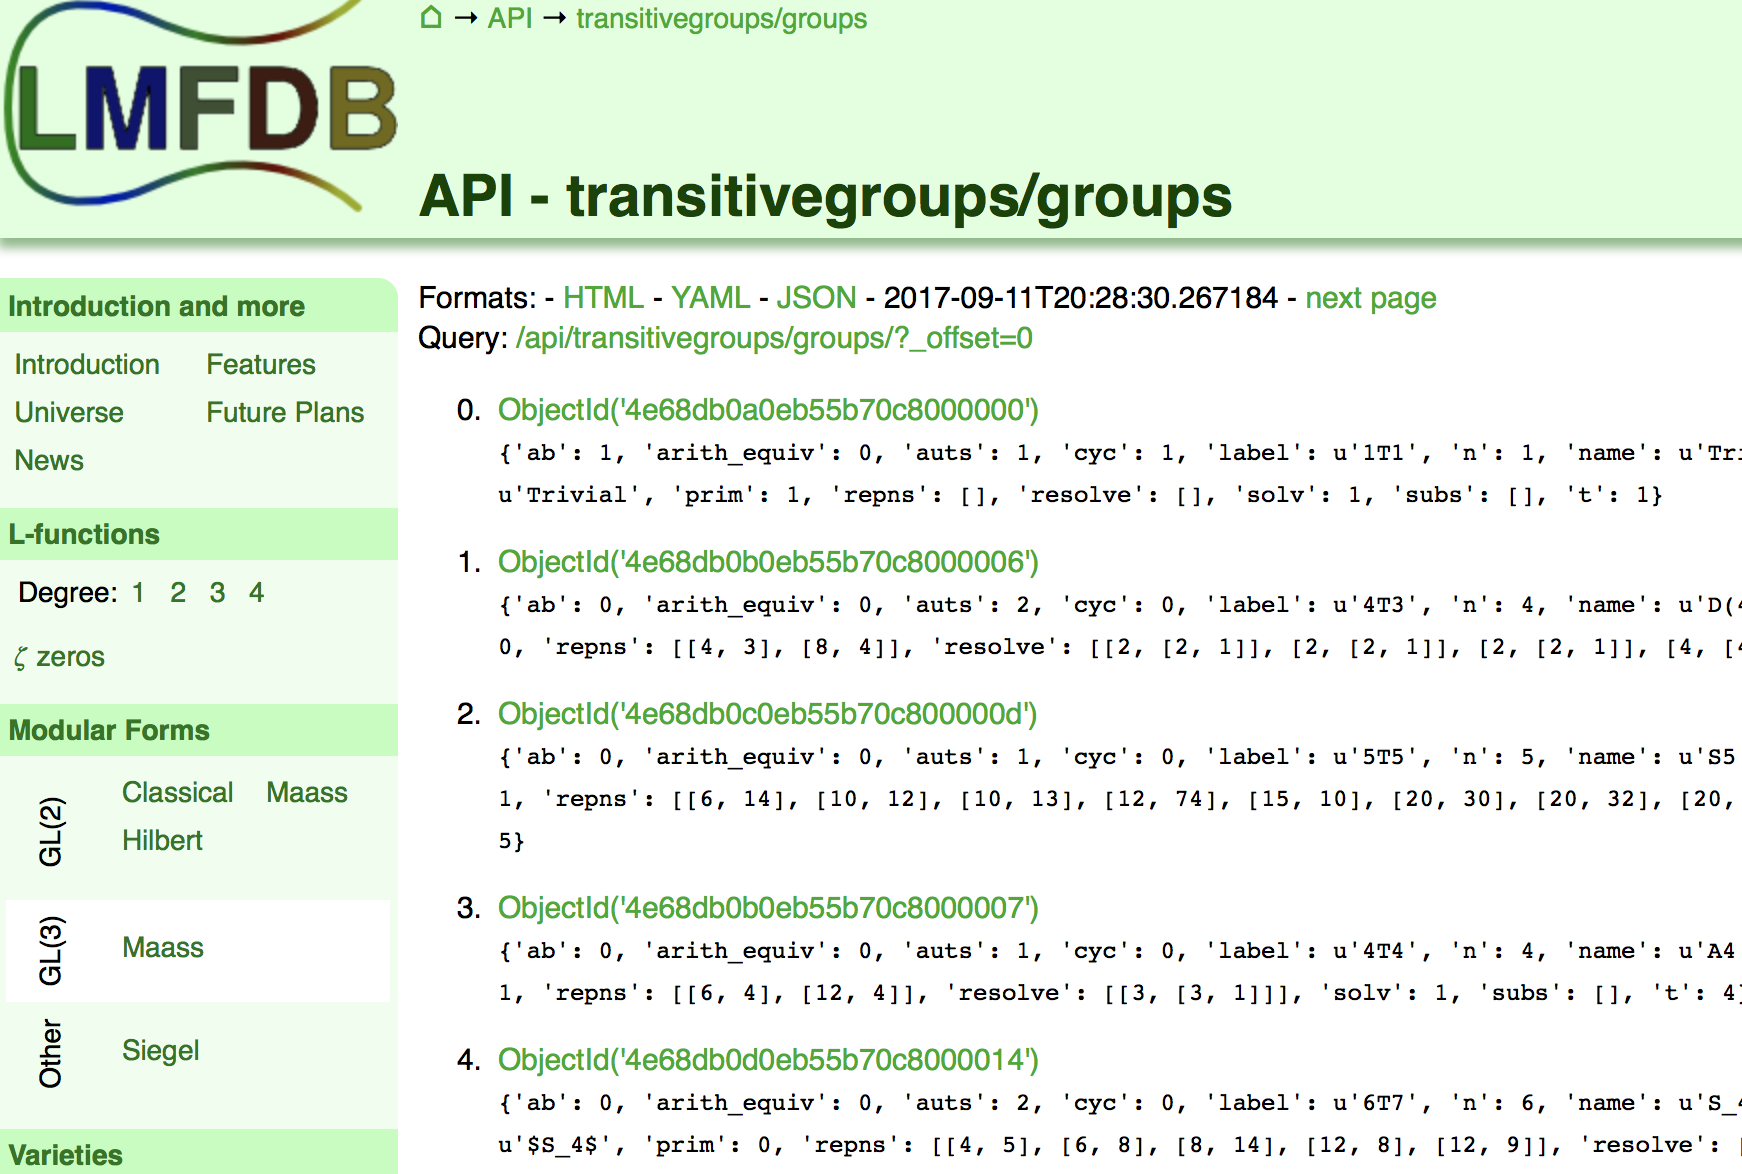
\includegraphics[width=\textwidth]{APIScreenshot.png}
  \end{center}

  \caption[The Web-Interface for the \lmfdb\ API. ]{
    The Web-Interface for the \lmfdb\ API. 
  }
  \label{fig:apiscreenshot}
\end{figure}
\ednote{Would like to show a search screenshot here, but since the lmfdb API breakage this is not possible. }
The \lmfdb\ API can be found at \ednote{cite url} and has two basic modes. 

In one mode, it is possible to make searches using the web-browser. 
Users can manually enter a query, and see a list of results displayed. 
A screenshot of this interface is shown in Figure~\ref{fig:apiscreenshot}. 
In a second mode, it is possible to request the results of the query directly as JSON. 
This can be used in automated scenarios. 

However both of these approach require queries to be formulated in a specific format.
For example, to search for all abelian elliptic cuves, the person querying \lmfdb needs to first encode this query. 
They need to realize that the \identifier{ab} key corresponds to the abelian property. 
Next, they need to realize that the property is boolean -- it's value is either \inlinecode{true} or \inlinecode{false}. 
Furthermore, \inlinecode{true} corresponds to $1$, and \inlinecode{false} corresponds to $0$. 
This information can then be used to make the query \inlinecode{?ab=1} to find all abelian transitive groups. 

In this example, each of the steps are relatively straightforward. 
In a general setting, e.g. when all elliptic curves with a specific isogeny matrix are sought for, this is no longer as simple. 
Moreover, this API has the problem that to use it one needs to be familar with both the mathematical background and the internal structure of \lmfdb. 

%%% Local Variables:
%%% mode: latex
%%% TeX-master: "paper"
%%% End:
